\chapter{Conclusões} \label{cap:conclusao}

%%% ---
%%% TODO List
%%% Fazer um levantamento do background dos problemas
%%% Italo na uff que mexeu no MLP junto com Rosseti
%%% Alterar para Revisão de literatura e conceituação teórica
%%% ---

% \section{LCRVND} \label{sec:lcrvnd}

LCRVND é um processo de busca local com exploração simultânea de múltiplas estratégias de vizinhança.

\subsection{GRASP}\label{subsec:lcrvnd_grasp}

O GRASP \cite{feo:1989} no Algoritmo~\ref{alg:grasp} use o valor de $\alpha$ de 20\%.
Na linha~\ref{alg:grasp:createThreads} criamos as threads CPU para os processos (usando a tecnologia OpenMP), o número total de iterações utilizado para o GRASP é de $maxIterations \times maxThreads$, um produto no número de iterações pelo número de threads utilizadas.

\begin{algorithm}[htpb]
\caption{GRASP}
\label{alg:grasp}
\begin{algorithmic}
    \Function{GRASP}{Rota: $x$, Itens selecionados: $y$, maxIterations}
        \Let{$(x^*,y^*)$}{$(x, y)$}
        \For{$counter \gets 1$ to $maxIterations$}
            \For{$threadId \gets 1$ to $maxThreads$} \label{alg:grasp:createThreads} \Comment{Cada thread CPU roda um CUDA stream}
                \For{$i \gets 1$ to $n$}
                    \Let{$candidateCities$}{$possibleCitiesFor(x_i)$}
                    \State $sort(candidateCities)$; \Comment{Ordenar as cidades pela distância da anterior}
                    \Let{$x_i$}{$randomlyChoose(candidateCities, \alpha)$} \Comment{Escolher uma das $\alpha$ mais próximas cidades}
                \EndFor
                
                \For{$i \gets 1$ to $m$}
                    \Let{$y_i$}{$rand()$} \Comment{Seleciona os itens aleatoriamente}
                \EndFor
                
                \Let{$(x', y')$}{$LCRVND(small, x, y)$}
                \If{$ value(x', y') > value(x^*, y^*) $}
                    \Let{$(x^*, y^*)$}{$(x', y')$}
                \EndIf
            \EndFor
        \EndFor
        \Let{$(x',y')$}{$LCRVND(large, x^*, y^*)$}
        \Return{$(x',y')$}
    \EndFunction
\end{algorithmic}
\end{algorithm}

\subsection{Busca local}\label{subsec:lcrvnd_localSearch}

O processo de busca local proposto é uma melhoria da busca local apresentada em~\cite{araujo:2009}.
Essa abordagem usa uma busca local que mantém os $L_{max}$ melhores soluções encontradas numa lista, então o processo seleciona a melhor solução não marcada, a marca e enumera seus vizinhos para uma determinada vizinhanças.
A propriedade paralela do método torna o uso da arquitetura GPU uma boa escolha para sua implementação~\footnote{Para sua implementação foi usada a API CUDA\texttrademark da NVIDIA\texttrademark.}
Uma GPU consiste de um conjunto de stream multiprocessors com centenas de unidades de processamento executando instruções Single Instruction Multiple Threads (SIMT). Nesse paradigma, para atingir boa performance é necessário executar operações similares sobre todos os conjuntos de dados no mesmo multiprocessador, o que é bem explorado pela metaheurística baseada em busca locar em~\cite{Coelho:2017}. 
Um aspecto diferenciado é que cada vizinhança pode ter tamanhos diferentes, dessa forma para obter um melhor uso da placa gráfica é útil fazer uso da tecnologia de paralelismo dinâmico.%~\cite{DiMarco:2013}.

\begin{algorithm}[htpb]
\caption{LCRVND}
\label{alg:lrcvnd}
\begin{algorithmic}[1]
    \Function{LCRVND}{Rota: $x$, Itens selecionados: $y$}
        \Let{$L$}{$\{ (x, y) \}$} \Comment{Solução inicial}
        \While{$\exists\;(x',y') \in L \mid (x',y')$ não marcado $\land$ melhor solução não melhorou nas últimas $iterMax$ iterações}
            \State $marcar(x',y')$
            \For{$\lambda \in \Lambda$}
                \Let{$L'$}{$\lambda(x',y')$} \label{alg:lrcvnd:dynamicParalelism} \Comment{$L'$ lsita de soluções para a vizinhança $\lambda$}
                \Let{$L$}{$L \cup L'$} com $|L|=listSize$; \Comment{Lista de soluções ordenada}
            \EndFor
        \EndWhile
        \Return{Melhor solução em $L$}
    \EndFunction
\end{algorithmic}
\end{algorithm}

Todo o processo no Algoritmo~~\ref{alg:lrcvnd} roda na GPU, a linha~\ref{alg:lrcvnd:dynamicParalelism} faz uma chamada para um kernel~\footnote{Kernel é uma função com múltiplas threads (geralmente milhares) que executam na GPU.} considerando o tamanho da vizinhança na configuração de lançamento.
Para representação da solução são utilizados dois vetores $x$ e $y$, sendo $x$ um vetor de inteiros representando a rota e $y$ um vetor de booleano indicando se cada item deve ser coletado na sua cidade ou não.

\begin{figure}[htbp]
    \centerline{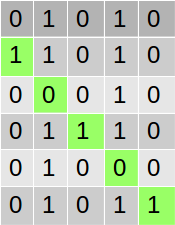
\includegraphics[scale=0.4]{figuras/pmv/notBit.png}}
    \caption{Operador de negação de bit.}
    \label{fig:operadorNegacaoBit}
\end{figure}

Para as vizinhanças da solução foram usados dois tipos de operações, uma sobre $x$ e outra sobre $y$, em $x$ foram usados 4 tipos de operações descritos a seguir, ao passo que para $y$ foram usadas duas operações, o operador de Negação de Bit (coletar um item se não estiver presente ou deixar de coletá-lo caso contrário, exemplificado na Figura~\ref{fig:operadorNegacaoBit}).
Em resumo, a combinação dos movimentos em $x$ e $y$ geram 8 vizinhanças diferentes.
Nessa abordagem, cada solução possui muitos vizinhos, sendo o total calculado pela Equação.~\eqref{eq:neighboorSize}.

\begin{equation} \label{eq:neighboorSize}
    |\Lambda(x, y)| = \frac{4nm(n - 1)}{2} + \frac{4n(n - 1)}{2} = 2n(n - 1)(m + 1) = \Theta(m\;n^2)
\end{equation}

\label{subsec:localSerach:neighborhoods}
As operações na rota $x$ possuem $\frac{n (n -1)}{2}$ vizinhos, a operação de Troca (Swap, Figura~\ref{fig:operadorSwap}) consiste de trocar cada par de inteiros no vetor, outrossim a operação 2-Opt consiste em reverter um grupo de elementos formado por cada par de inteiros do vetor.
A operação de Shift consiste de mover todos os elementos uma posição para a esquerda (Figura~\ref{fig:operadorShiftLeft}) ou direita (Figura~\ref{fig:operadorShiftRight}) dentro de um par de elementos.

\begin{figure}%
    \centering
    \subfloat[Troca]{{
        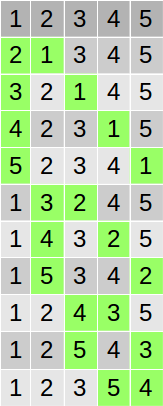
\includegraphics[scale=0.4]{figuras/pmv/swap.png}
        \label{fig:operadorSwap}
    }}%
    \qquad
    \subfloat[Inversão]{{
        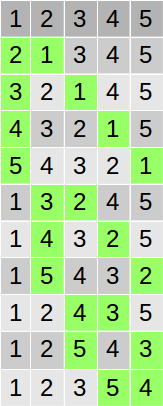
\includegraphics[scale=0.4]{figuras/pmv/inversion.png}
        \label{fig:operadorInversion}
    }}%
    \caption{Vizinhanças troca e inversão}%
    \label{fig:swapInversion}%
\end{figure}

\begin{figure}%
    \centering
    \subfloat[Shift left]{{
        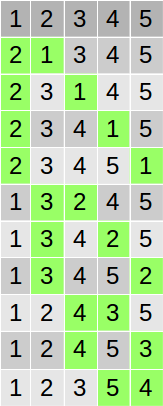
\includegraphics[scale=0.4]{figuras/pmv/shiftLeft.png}
        \label{fig:operadorShiftLeft}
    }}%
    \qquad
    \subfloat[Shift right]{{
        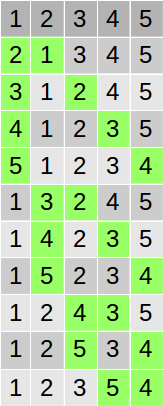
\includegraphics[scale=0.4]{figuras/pmv/shiftRight.png}
        \label{fig:operadorShiftRight}
    }}%
    \caption{Vizinhanças Shift}%
    \label{fig:shiftLeftRight}%
\end{figure}


Foi possível simular uma memória global em um dataflow pelo uso do nó de \textit{flip-flop} apresentado na Seção~\ref{subsec:flipFlop} de forma a prover uma memória para o nó \textit{man} do grafo dataflow do DVND, expresso na Figura~\ref{fig:dvndGraph}.

Conforme discutido na Seção~\ref{subsec:multiplasSaidas}, foi proposta a melhoria da biblioteca \textit{Sucuri} para que os nós de seus grafos comportem múltiplas portas de saída, sendo visto na Seção~\ref{sec:resultadosMultiplasPortas} que os resultados indicam sua eficiência para instâncias com tamanho maior ou igual a 318.

\section{RVND}

Foi discutido na Seção~\ref{sec:resultadosRVND} que em termos de melhoria na qualidade da solução não foi encontrada grande diferença nos métodos RVND em sua implementação clássica e da implementação em dataflow.

Em termos de tempo de execução houve uma pequena diferença em algumas instâncias pesando para a implementação dataflow e em outras para a implementação clássica.

\section{DVND}

No que diz respeito a comparação entre o DVND implementado em dataflow e a implementação original podemos ver que a versão clássica apresentou melhores tempos para as menores instâncias, sendo alcançado pela tempo da implementação em dataflow apenas na instância 5, de tamanho 657.
Apenas na instância 7 (tamanho 1001) o DVND em dataflow conseguiu melhorar o tempo do DVND clássico, contudo a melhoria dos resultados com o aumento do tamanho da solução indica que o mesmo possui tempo de execução mais controlado para grandes instâncias.

Em termos de valor da solução encontrada pode se ver na discussão da Seção~\ref{sec:resultadosDVND} que o DVND clássico conseguiu melhorar mais a solução inicial quando comparado à implementação em dataflow.

É importante ressaltar que tanto a implementação clássica quanto a implementação em dataflow do DVND melhoraram o tempo de execução quando comparadas ao RVND dataflow ou mesmo o clássico.

\section{GDVND}

Desta forma foi possível mostrar que o GDVND consegue diminuir a necessidade de explorar vizinhanças pois, conforme discutido na Seção~\ref{sec:gdvndTimeMan}, o tempo gasto por esse na exploração de vizinhanças é menor para as maiores instâncias, contudo carece de uma melhor estratégia para combinar os movimentos pois este está tomando uma parte significativa do tempo de execução do procedimento como um todo.

% \section{DVND} \label{sec:dvndClassico}

O \textit{Distributed Variable Neighborhood Descent} DVND concebido por~\cite{RIOS201839} utiliza múltiplas vizinhanças conforme o faz o VND (\textit{Variable Neighborhood Descent} proposto por \cite{mladenovic1997}) contudo propõe o processamento das vizinhanças de forma distribuída.
Este processamento distribuído se dá pelo escalonamento das tarefas de enumeração das vizinhanças o que naturalmente proporciona a aleatoriedade proposta no RVND.

A implementação em dataflow não pode alcançar uma grande melhoria do RVND em termos de tempo ou qualidade da solução pois o grafo se assemelha a uma cascata (veja a Figura~\ref{fig:rvndGraph}) o que não permite alcançar paralelismo, então se torna natural o uso do método DVND conforme o Algoritmo~\ref{alg:dvnd}. 
A ideia do DVND é que quando uma solução atinge um ótimo local para uma estrutura de vizinhança ainda pode existir um vizinho com melhor valor de função objetivo em uma estrutura de vizinhança diferente, destarte não necessariamente sendo um ótimo local para todas as vizinhanças
Se uma melhoria é encontrada o processo de busca é reiniciado para todas as estratégias de vizinhança.

\begin{algorithm}[htpb]
\caption{DVND clássico}\label{alg:dvnd}
\begin{algorithmic}[1]
    \Function{DVND}{Solução: $s$, Vizinhanças: $N$}
        \Let{$W$}{$\emptyset$}
        \Let{$H$}{$\emptyset$}
        \ForAll{$N_k \in N$}
            \Let{$s_k$}{$s$} \Comment{Solução atual para vizinhança $k$}
            \Let{$H_{k,s}$}{$true$} \Comment{Solução já foi enumerada pela vizinhança}
            \Let{$W_k$}{$false$} \Comment{Vizinhança aguardando solução}
            \State Chame de forma assíncrona $N^k(s_k)$
        \EndFor
        
        \While{$\exists w \in W \mid w = false$}
            \Let{$k$}{join $N^k(s_k)$} \Comment{Aguarda a resposta da vizinhança $N^k$}
            \Let{$s_k$}{Melhor solução de $N^k(s_k)$}
            \If{$f(s_k) < f(s)$}
                \Let{$s$}{$s_k$}
            \EndIf
            
            \Let{$W_k$}{$true$}
            \ForAll{$N_k \in N$}
                \If{$W_k \land \neg H_{k,s}$}
                    \Let{$s_k$}{$s$}
                    \Let{$H_{k,s}$}{$true$}
                    \Let{$W_k$}{$false$}
                    
                    \State Chame de forma assíncrona $N^k(s_k)$
                \EndIf
            \EndFor
        \EndWhile
        \Return{$s$}
    \EndFunction
\end{algorithmic}
\end{algorithm}

Considerando $ \mathcal{M} = M^{DVND} = M^1 \cup M^2 \cup \dots \cup M^k $ o conjunto com os movimentos de todas as vizinhanças usadas pelo DVND, então em termos de movimento temos que a solução $s''$ retornada a cada iteração do DVND pode ser escrita como $s'' = m_z \circ s$ com $m_z \in \mathcal{M}$ e $\widehat{m_z}(s) < \widehat{m_i}(s) \mid \forall m_i \in \mathcal{M}$.
Vale ressaltar que $\mathcal{M} = M^{DVND} = M^{RVND}$, a diferença dos métodos é que a cada iteração o RVND move para a melhor solução da vizinhança atual e no caso do DVND este move para a melhor solução entre todas as vizinhanças.

% Igor, o que acha dessa afirmação?
Numa análise em mais alto nível do RVND (Algoritmo~\ref{alg:rvnd}) e DVND (Algoritmo~\ref{alg:dvnd}), pensando-se à luz das estratégias de \textit{First improvement} e \textit{Best improvement}, o RVND enumera as soluções vizinhas da solução atual vizinhança por vizinhança até encontrar uma solução que a melhore e então retorna para a primeira vizinhança ao passo que o DVND enumera todas as vizinhanças para então optar pela solução de melhor valor.
Desta forma o RVND é uma estratégia de \textit{first improvement} no contexto de vizinhanças de solução e o DVND uma estratégia de \textit{best improvement}.


\section{Propostas futuras}

\subsection{Testar com instâncias maiores} \label{subsec:instanciasMaiores}

No intuito de verificar melhor o desempenho do método dataflow DVND e sua escalabilidade uma prova de conceito imaginada pra ser utilizada é a realização de teste computacionais para instâncias maiores, tendo em vista a comparação de resultados com instâncias do clássico PCV.

\subsection{Decomposição de vizinhanças} \label{subsec:decomposicaoVizinhancas}

Conforme descrito na seção~\ref{subsec:metodologiaDecomposicaoVizinhancas}, as vizinhanças exploradas nos problemas não são indivisíveis, desta forma uma maneira de proporcionar maior paralelismo pode ser feita através da decomposição das destas em sub vizinhanças de forma a serem exploradas paralelamente.

Acredita-se que a decomposição de vizinhanças aliada a composição de movimentos pode proporcionar um grande ganho em termos de qualidade da solução uma convergência muito mas rápida ao serem aplicados mais de um movimento simultaneamente, melhorando assim o tempo da busca local que em geral é a etapa mais custosa em termos computacionais para o processo de solução de um problema de otimização.

% \subsection{Publicações e Cronograma}

Etapas deste trabalho já foram publicadas nas conferência International Conference on Variable Neighborhood Search (ICVNS) e publicado na edição especial do Electronic Notes in Discrete Mathematics (ENDM), também sendo publicado na conferência Parallel Programming Models (MPP), realizado em conjunto com o 32nd IEEE International Parallel and Distributed Processing Symposium (IPDPS). Existe um draft para submissão no Computers \& Operations Research, que irá englobar resultados da união de movimentos.

% ... Escrever um pouco melhor.
A etapa inicial do trabalho, apresentada no ICVNS, diz respeito ao método descrito na seção~\ref{sec:lcrvnd} e resultados apresentados na seção~\ref{sec:res_lcrvnd}.
A proposta apresentada no MPP é detalhada na seção~\ref{sec:df_dvnd} e seus resultados analisados em~\ref{sec:res_df_dvnd}.

O cronograma esperado é desenvolver a proposta e fechar antes do prazo regular do mestrado (Outubro/2018), com meta de terminar ainda em Agosto/2018 para inscrição imediata e entrada em programas de doutorado da região.
